\documentclass[11pt]{article}

% ------------------ PACKAGES ------------------
\usepackage[a4paper, margin=1in]{geometry}
\usepackage{amsmath, amssymb}
\usepackage{graphicx}
\usepackage{hyperref}
\usepackage{cite}
\usepackage{enumitem}
\usepackage{authblk}  % for author/affiliation formatting

% ------------------ METADATA ------------------
\title{Exstream: implementation and improvements}
\author[1]{Remi Guillou}

% ------------------ DOCUMENT ------------------
\begin{document}

\maketitle

\section{Introduction}
Exstream is an anomaly explanation tool for time series data created in 2017\cite{Exstream_origin}. It was designed to use entropy to measure the segmentation of normal and anomalous points for each feature and outputting a score between 0 and 1. Based on these scores, it selects a number of features to explain the anomaly. This method has gone through several iterations, improvements and changes to its implementation. This paper aims to document the current state of Exstream while also providing insights into its evolution and the rationale behind its design choices.


\section{Original paper}
The original paper \cite{Exstream_origin} introduces the scoring mechanism and some feature filtering techniques.
\subsection{Scoring}
We obtain a score from 0 to 1 for each feature. The score is computed as follows:
Let $TS_a$ and $TS_r$ be respectively the anomalous and reference time series. Then $|TS_a|$ and $|TS_r|$ are their number of points.\\
First we sort all the points by their value. We then obtain pure intervals from the sorted points. This means intervals that contain only points from one of the two types. There can also be mixed intervals, which contain points from both types. This happens if both normal and anomalous points take some specific values. Let $n$ be the number of segments, and $p_i$ represent the ratio of data points included in the ith segmentation.\\
Let $p_a = \frac{|TS_a|}{|TS_a| + |TS_r|}$ and $p_r = \frac{|TS_r|}{|TS_a| + |TS_r|}$ be the proportions of anomalous and reference points respectively.\\
First we compute the class entropy: 
\begin{equation}
    H_{class} = p_a \log(\frac{1}{p_a}) + p_r \log(\frac{1}{p_r})
\end{equation}
Next the segmentation entropy is computed as follows:
\begin{equation}
    H_{segmentation} = \sum_{i=1}^{n} p_i \log(\frac{1}{p_i})
\end{equation}
The mixed segments receive a penalty to be added to the segmentation entropy. This penalty is defined as the entropy of the "worst" segmentation between these points. Let us call it $H_{segmentation}(c*)$.\\
The final segmentation entropy is then:
\begin{equation}
    H_{segmentation}^{+} = H_{segmentation} + \sum_{j=1}^{m} H_{segmentation}(c_j*)
\end{equation}
Finally, the score is computed as follows:
\begin{equation}
    D(f) = \frac{H_{class} }{H_{segmentation}^{+}}
\end{equation}
This gives us a score between 0 and 1, where 0 means the feature is not useful for explaining the anomaly, and 1 means it is very useful.

\begin{figure}[h!]
    \centering
    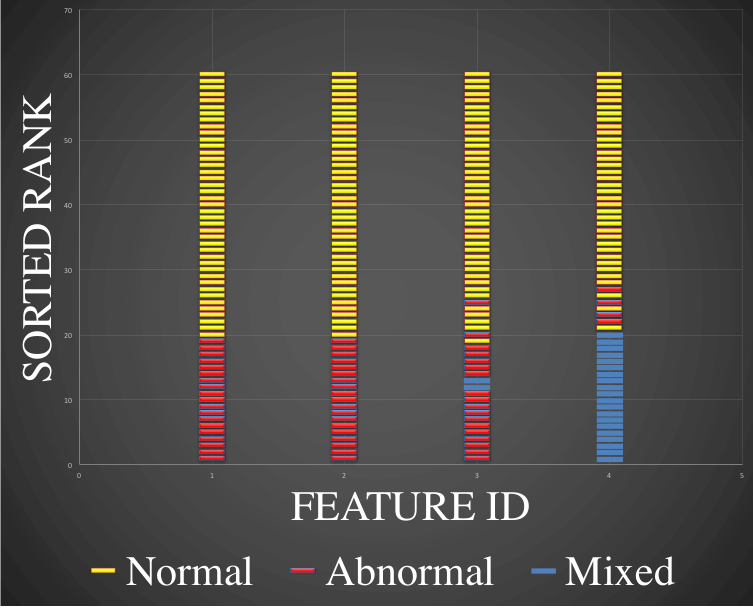
\includegraphics[width=0.3\textwidth]{images/exstreamplot.png}  % Replace with your image filename
    \caption{Feature segmentation example.}
    \label{fig:exstream_segments}
\end{figure}


\subsection{Feature filtering}
A short explanation is prefered. To this end, the score of every feature isn't returned to the user. Therefore, we need to filter the features to keep only the most useful ones. The original paper proposes three methods:

\begin{enumerate}
    \item \textbf{Reward Leap Filtering}:
    Features are ranked using an entropy-based single-feature reward. The system detects sudden drops (leaps) in the reward values, and only retains features ranked above the largest leap. This filters out low-reward, potentially uninformative features.

    \item \textbf{False Positive Filtering}:
    Features with high rewards are further validated across related partitions (e.g., other executions of the same job). Features that also exhibit high reward in unrelated or normal scenarios are considered false positives and removed.

    \item \textbf{Correlation Clustering}:
    Remaining features are clustered based on pairwise correlation. Highly correlated features (e.g., duplicates or near-duplicates) are grouped together, and only a single representative feature is retained from each cluster to reduce redundancy in the final explanation.
\end{enumerate}

\section{Implementation}
There are two main implementations of Exstream. The first is stored in the \textit{exathlon-private} repository \cite{exathlon-private}. (created in November 2nd 2021). This incorporates the exstream method into the Exathlon pipeline \cite{Jacob2021Exathlon}. The second more recent is stored in the \textit{exathlon-explanation} repository \cite{exathlon-explanation} (created in October 25th, 2024). This is a standalone implementation of Exstream, which can be used independently to Exathlon and to any anomaly detection system. Both implementations are written in Python and use the same core algorithm. We will now describe this algorithm in more detail and the functions it makes use of.


\subsection{Structure}
The Exstream implementation is structured around a class called \texttt{Exstream}. The file containing the class is stored at the following path:\\
 \texttt{exathlon/explanation/explainers/data\_explainers/exstream\_origin.py} in the \textit{exathlon-explanation} repository and \texttt{src/exstream/exstream\_fp.py} in the \textit{exathlon-explanation} repository.
 This class contains two main methods:
\begin{itemize}
  \item \texttt{\_fit}:This method can be used to fit the model using the training data if needed. It is not used in the first version of Exstream, but it is included for compatibility with the Exathlon pipeline.
  \item \texttt{predict\_instance}: This methods takes as input an array of normal points (the reference time series) and an array of anomalous points (the anomalous time series). It returns an explanation in the form of a dictionary in the following format:
\begin{verbatim}
          {
            "feature_to_importance": {3: 0.5, 0: 0.2},
            "feature_to_intervals": {
                3: [(-inf, 0.2, False, True), (0.8, inf, True, False)],
                0: [(1, 2.2, True, True)]
            },
        }
\end{verbatim}
\end{itemize} 
In \textit{exathlon-explanation} it also contains some helper functions. However, helper functions are mostly stored in a different file stored at: \\
\texttt{exathlon/explanation/explainers/data\_explainers/helpers/exstream.py} in the \textit{exathlon-private} repository and \texttt{src/exstream/utils/helpers\_penalty.py} in the \textit{exathlon-explanation} repository.\\



\subsection{Scoring}
The scoring component of EXstream measures how well each feature explains the difference between normal and anomalous data points. It does so by computing a score that compares the class entropy with the segmentation entropy of the data when sorted by feature values. The score ranges from 0 to 1, where a score closer to 1 indicates that the feature offers strong explanatory power. The following subsubsections describe the core functions used for computing this score.

\subsubsection{get\_feature\_segments}

This function takes in the values of a feature for normal and anomalous data points and returns three sets of segments:
\begin{itemize}
  \item \textbf{Normal segments}: intervals containing only normal values,
  \item \textbf{Anomalous segments}: intervals containing only anomalous values,
  \item \textbf{Mixed segments}: intervals containing values from both sets.
\end{itemize}

The function first computes the set of common values between the normal and anomalous sets. It labels each point with:
\begin{itemize}
  \item $1$ if it appears only in normal data,
  \item $-1$ if it appears only in anomalous data,
  \item $0$ if it appears in both.
\end{itemize}

All values are then concatenated and sorted. Ranges of consecutive labels are identified using a helper function, and their corresponding value intervals are collected. The segments are returned as a list of tuples of the form:
\[
(\text{min\_value}, \text{max\_value}, \text{count})
\]
for each of the three segment types.

\subsubsection{get\_reg\_segmentation\_entropy}

This function computes the segmentation entropy using all segments (normal, anomalous, and mixed). For pure segments (normal and anomalous), the segmentation entropy is:
\[
H_{\text{segmentation}} = -\sum_i \frac{c_i}{n} \log \left( \frac{c_i}{n} \right)
\]
where \( c_i \) is the count of points in the $i$-th segment and \( n \) is the total number of records.

For mixed segments, a regularization penalty is added:
\[
\text{Penalty} = \sum_j \log(c_j)
\]
where \( c_j \) is the number of points in the $j$-th mixed segment. This penalizes features that do not cleanly separate the classes.

The final regularized segmentation entropy is:
\[
H^+_{\text{segmentation}} = H_{\text{segmentation}} + \text{Penalty}
\]

If no pure segments exist (i.e., all segments are mixed), the function returns \( +\infty \), indicating no separation power.





\subsubsection{get\_single\_feature\_reward}

This function computes the final reward score for a single feature. It takes as input:
\begin{itemize}
  \item The feature values for normal and anomalous data,
  \item The corresponding normal, anomalous, and mixed segments,
  \item The total number of records (optional).
\end{itemize}

It first calculates the class entropy:
\[
H_{\text{class}} = -p_n \log p_n - p_a \log p_a
\]
where \( p_n \) and \( p_a \) are the proportions of normal and anomalous points, respectively.

Then, it calls \texttt{get\_reg\_segmentation\_entropy} to compute the regularized segmentation entropy \( H^+_{\text{segmentation}} \). The final reward score is defined as:
\[
\text{Score}(f) = \frac{H_{\text{class}}}{H^+_{\text{segmentation}}}
\]
If all points belong to mixed segments, the denominator becomes infinite, and the score is set to 0.
\subsection{Feature Filtering}

Once the explanatory scores for each feature are computed, EXstream applies a sequence of filtering techniques to reduce redundancy, eliminate misleading features, and generate concise explanations. These techniques aim to retain only the most informative and distinct features. The implementation includes the following filtering steps.






\subsubsection{False Positive Filtering (get\_fp\_features)}

The function \texttt{get\_fp\_features} is used to eliminate features that exhibit false positive behavior. This behavior corresponds to those that show significant variability or monotonic trends even in normal data. The filtering is performed in an unsupervised manner and consists of two criteria:

\begin{itemize}
  \item \textbf{High variance}: Feature-wise standard deviations are computed and standardized using \texttt{StandardScaler}. Any feature whose scaled standard deviation exceeds a user-defined threshold \textit{scaled\_std\_threshold} is marked as a false positive.
  \item \textbf{Monotonic trends}: For each feature, the function computes the average value in non-overlapping sliding windows of length 5. If the sequence of these averages is strictly increasing or decreasing, the feature is also flagged as a false positive.
\end{itemize}

This step ensures the removal of features that are noisy or time correlated. Notably, if a feature is only increasing then it will always get a high score however isn't a satisfying explanation.

\subsubsection{Reward Leap Filtering (get\_low\_reward\_features)}

The \texttt{get\_low\_reward\_features} function implements the reward leap filtering method described in the original EXstream paper. The idea is to discard features with low explanatory power by analyzing the distribution of reward scores. The implementation proceeds as follows:

\begin{enumerate}
  \item Sort all reward scores in descending order.
  \item Compute the differences (leaps) between adjacent sorted scores.
  \item Identify the maximum leap: this represents the point of sharpest reward drop.
  \item Use the reward value \textit{before} this leap as a threshold.
  \item Mark all features with scores below this threshold as low-reward and return them.
\end{enumerate}

This method assumes a large drop off in scores between the best scoring features and the rest. If all scores are regularly distributted, this method will not filter correctly the features. However, in general this isn't the case and we do observe a large drop off in scores between the best features and the rest. Overall, this filtering step helps to keep only the most informative features that contribute significantly to the anomaly explanation. It often provides a good balance between explanation length and informativeness, especially in cases where some features have high separation power.






\subsubsection{Correlation Clustering (get\_clustered\_features)}

The final step groups redundant features using Pearson correlation and removes duplicates. The function \texttt{get\_clustered\_features} performs the following operations:

\begin{itemize}
  \item Computes the pairwise Pearson correlation matrix between features.
  \item Converts correlations into distances using the transformation: \( d_{ij} = 1 - |r_{ij}| \).
  \item Applies hierarchical clustering using complete linkage on the resulting distance matrix.
  \item Flattens the cluster hierarchy using half the maximum distance as the cophenetic threshold.
\end{itemize}

Each resulting cluster groups features that are highly correlated in absolute value. A single representative feature can be selected per cluster to minimize redundancy in the final explanation. This clustering improves interpretability by avoiding explanations with multiple variants of the same signal.





\section{Improvements}

Since the original paper, several improvements have been made to the Exstream implementation. In this part we will explore new improvements that have been made to the Exstream method as well as fixes to the implementation.

\subsection{Sample selection}
Originally, Exstream was designed to work with the entire time series. This means that to create an explanation, it uses the entire anomalous interval as well as all normal points directly preceding it. This may lead to several issues. First, the separation between normal and anomalous points may be noisy. Even on ground truth samples, annotation errors may appear. This is even more true for real world data where we rely on a detection model to provide us with the intervals. This may lead to incorrect explanations. Second, the normal points preceding the anomaly may not be representative of the normal behavior. This would lead to the wrong features being selected. 
In this part we will explore methods that were implemented to address these issues.

\subsubsection{Removing Edges of intervals}
The first and easiest method to implement is to remove the edges of both the normal and anomalous intervals \cite{Remi_thesis}. This introduces a hyperparameter that defines the percentage of points to remove from each side of the intervals. In practice this removes the most uncertain points where the segmentation is high. This lead to higher scores for some explanations and more robust feature selection.
This was implemented in the Exathlon pipeline \cite{exathlon-private} by removing the sample of points at the beginning of the \textit{predict\_instance} function in the Exstream class.




\subsubsection{Gaussian weight scaling}
Another option to reduce randomness in results due to the edge points is to weight the points in the intervals. This weight is then used to compute the score. Points with higher weights contributing higher than those with low weights. This was done using a Gaussian distribution centered on the middle of the interval \cite{Mija_thesis}.



The gaussian scores are computed using two functions: 
\paragraph{get\_gaussian\_time\_score}
This function assigns a weight to a point based on its position within an interval.
\paragraph{Inputs}
\begin{itemize}
  \item \texttt{position} is the position of the point inside the interval,
  \item \texttt{interval\_length} is the total number of points in the interval,
  \item \texttt{sigma} controls the standard deviation \( \sigma \) by dividing the interval length (default: 35.0),
  \item \texttt{beta} is the shape parameter of the generalized Gaussian (default: 10).
\end{itemize}

The midpoint \( \mu \) is computed as \( \texttt{interval\_length} / 2 \), and the standard deviation is derived as \( \sigma = \texttt{interval\_length} / \texttt{sigma\_scale} \). The final weight is then given by:

\[
w(i) = \exp\left( - \left| \frac{i - \mu}{\sigma} \right|^{\beta} \right)
\]

This function ensures that points near the interval center receive weights close to 1, while boundary points receive exponentially smaller weights.

\paragraph{get\_points\_val\_idx\_scores}

This function processes either normal or anomalous points and prepares them for entropy scoring. Its inputs include the data array and a set of binary ranges (each corresponding to a detected anomaly or normal segment). It returns a list of triplets:

\[
(\texttt{value}, \texttt{index}, \texttt{gaussian\_score})
\]

For each point:
\begin{enumerate}
  \item The interval length is computed.
  \item The point’s relative position \( i \) is used to compute a Gaussian weight via \texttt{get\_gaussian\_time\_score}.
  \item The resulting weight is stored alongside the value and index.
\end{enumerate}

These scores are not directly used in computing the class entropy but are passed to downstream processing functions such as \texttt{update\_points\_bin} and \texttt{update\_points\_categorical}, where they influence which points are retained, discarded, or downsampled.



\subsubsection{Gaussian-weighted downsampling in bins}
\label{sec:gaussian-downsampling}

After points are assigned a temporal weight, marginal, low-weight samples are filtered out.  
This is handled by \texttt{update\_points\_bin}, which (i) groups values into uniform bins, (ii) filters or
down-samples mixed bins according to cumulative Gaussian weight, and (iii) classifies each bin as \emph{normal}, \emph{anomalous}, or \emph{mixed}.  
This is done in the following way:

\paragraph{Inputs}
\begin{itemize}
  \item \texttt{normal\_points\_info}, \texttt{ano\_points\_info}: lists of triplets
        $(v,\;i,\;w)$ where $v$ is the feature value, $i$ its original index, and
        $w$ the Gaussian weight.
  \item \texttt{n\_bins}: number of equi-width bins.
\end{itemize}
\paragraph{Outputs}
\begin{itemize}
  \item filtered / down-sampled point lists;
  \item \texttt{bins\_info}: tuples $(c,\min v,\max v)$ with
        $c\!\in\!\{1,-1,0\}$ for pure normal, pure anomalous, or mixed bins.
\end{itemize}

\paragraph{Step\,1 Bin initialisation}
\begin{enumerate}[label=\arabic*.]
  \item Compute global minimum and maximum:
        $\min v,\max v$ over \texttt{normal} $\cup$ \texttt{anomalous}.
  \item Generate $\texttt{n\_bins}$ uniform edges
        $\{b_0,b_1,\dots,b_{\texttt{n\_bins}}\}$
        with $b_{\texttt{n\_bins}} \leftarrow b_{\texttt{n\_bins}}+0.1$
        to guarantee right-open inclusion of the maximum value.
\end{enumerate}

\paragraph{Step\,2 Per-bin processing}  
For each interval $[b_j,b_{j+1})$:
\begin{enumerate}[label=\alph*)]
  \item \emph{Collect points.}
        \[
          S_N=\{(v,i,w)\!\in\!\texttt{normal} \mid b_j\le v<b_{j+1}\},\quad
          S_A=\{(v,i,w)\!\in\!\texttt{anom}\}
        \]
        Let $n_N=\lvert S_N\rvert$, $n_A=\lvert S_A\rvert$,
        $S_n=\sum_{S_N} w$, $S_a=\sum_{S_A} w$.
  \item \emph{Pure bins.}  
        If $(n_N>0, n_A=0)$ mark bin class $c\!=\!1$ (normal);  
        if $(n_A>0, n_N=0)$ mark $c\!=\!-1$ (anomalous).
  \item \emph{Mixed bins.}  ($n_N>0$ and $n_A>0$)
        \begin{enumerate}[label=\roman*.]
          \item \textbf{Low-weight removal.}  
                If $S_a<1$ discard all anomalous points;
                if $S_n<1$ discard all normal points.
          \item \textbf{Gaussian down-sampling.}  
                When both classes remain and at least one class
                has cumulative weight \(<\) its cardinality,
                iterate through points sorted by descending weight
                and create \emph{groups} whose accumulated score
                exceeds~1.  Replace each group by a single
                representative:
                \[
                  v_{\text{rep}}=\frac{1}{m}\sum_{k=1}^{m}v_k,
                \]
                preserving the first index of the group and setting
                its weight to \texttt{None}.  This yields at most
                \(\lceil S_{(\cdot)}\rceil\) representatives per class.
          \item Label the bin as mixed, $c\!=\!0$.
        \end{enumerate}
  \item Append $(c,b_j,b_{j+1})$ to \texttt{bins\_info}.
\end{enumerate}

\paragraph{Step\,3 Output}
Return the (possibly reduced) \texttt{normal\_points\_info},
\texttt{ano\_points\_info}, and the full \texttt{bins\_info} list.  
The latter feeds directly into \texttt{get\_segments} to build normal,
anomalous, and mixed value ranges for entropy computation
The segments are then created using the bins instead of the original points.




\paragraph{Benefits}
\begin{itemize}
  \item \textbf{Noise suppression}: bins whose cumulative weight is
        negligible are removed early.
  \item \textbf{Edge robustness}: Gaussian weighting prioritises
        central samples, down-weighting interval boundaries that are
        prone to labelling noise.
  \item \textbf{Computational efficiency}: replacing groups of similar,
        low-impact points by a single representative shrinks the data
        passed to subsequent entropy calculations without sacrificing
        explanatory power.
\end{itemize}


This design reduces sensitivity to interval boundaries and improves the robustness of explanations, especially in long anomalies or poorly aligned traces.
This was implemented in the standalone Exstream implementation \cite{exathlon-explanation}.


\paragraph{Fix to the Gaussian downsampling}
The first implementation \cite{Mija_thesis} of Gaussian downsampling lead to some scores being greater than 1. This was solved \cite{martineau2024exstream}.



\subsubsection{New point construction}
An attempt to generalize the normal points used in the explanation was made by sampling new normal points that are "close" to the anomalous ones \cite{Remi_thesis}. This is done using the anomaly detection model. Assuming the model used is an autoencoder, or at least makes use of a latent space. Normal points close to the anomalous points in the latent space would in theory be more representative and lead to better explanations.\\
However, in the case of the Exathlon dataset, the traces are taken from different executions and systems leading to "domains". These in turn lead to inherent differences from one trace to the other that isn't due to the anomaly. This in turn might lead to the explanation picking up features not linked to the anomaly but rather to the domain. \\
In our case, the latest detection model used is DIVAD. This model uses two latent space. One capturing the class information and the other the domain information. The idea was therefore to sample points close to the anomaly in the class latent space. We would then reconstruct the points in the right domain using the domain latent space of the original anomalous trace.

This was implemented in the Exathlon pipeline \cite{exathlon-private} by sampling the points in the \textit{predict\_instance} function of the Exstream class. 
\begin{figure}[h!]
    \centering
    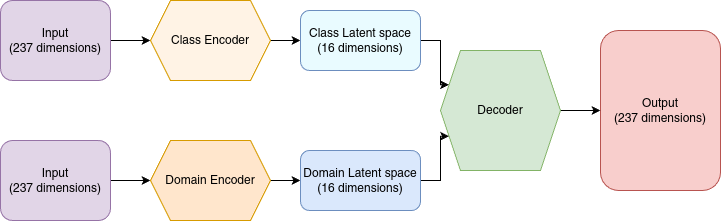
\includegraphics[width=0.5\textwidth]{images/divad_simple.png}  % Replace with your image filename
    \caption{DIVAD}
    \label{fig:divad}
\end{figure}


\subsection{Feature score}
The feature scoring from the original paper is simple and effective. Some improvements have however been made.

\subsubsection{Worse case segmentation entropy}
\label{sec:worst_case_segmentation_entropy}
The original paper doesn't specify exactly how the "worst case segmentation entropy" should be computed. In the original implementation \cite{exathlon-private}, it simply took the number of points in the mixed segment $n$. And added the following penalty:
\begin{equation}
    H_{segmentation}(c*) = \sum_{i=1}^{n} \frac{1}{n} \log(n)
\end{equation}
Which would be considering that every point is interleaved in the segment. However this is assuming there are as many normal and anomalous points in the segment. This is not always the case. For example if the mixed segment contains 8 normal points and 1 anomalous one, the worst case segmentation would be 4 normal followed by the 1 anomalous then by the 4 other normal points. This would lead to a penalty of:
\begin{equation}
    H_{segmentation}(c*) = \frac{4}{n} \log(n/4) + \frac{1}{n} \log(n) + \frac{4}{n} \log(n/4)
\end{equation}
Which in all cases ends up being lower than the original penalty. The only case where it is equal is when there are as many normal as anomalous points in the segment.  
Therefore in order to change this, two changes were made. First the get\_feature\_segments function now returns both the number of normal and anomalous points in each segment. This is then used in the get\_reg\_segmentation\_entropy function to compute the worst case segmentation entropy using a new function called compute\_mixed\_segm\_score in the following way:

If the two classes have equal counts, the function assumes a perfect alternation pattern and assigns the maximum possible mixed-segment score:
\[
H_{\text{mixed}} = (n_{\text{normal}} + n_{\text{anomalies}}) \cdot \frac{1}{N} \cdot \log N
\]

In the more general case, the class with more points is split into groups that are inserted between the smaller class's instances, creating an optimally mixed sequence. Let:
\begin{itemize}
  \item \( s = \min(n_{\text{normal}}, n_{\text{anomalies}}) \),
  \item \( l = \max(n_{\text{normal}}, n_{\text{anomalies}}) \),
  \item \( N \text{ is the number of points}\)
\end{itemize}

We then compute:
\begin{itemize}
  \item The number of base-sized groups \( g_1 = \left\lfloor \frac{l}{s + 1} \right\rfloor \),
  \item The number of larger groups \( g_2 = g_1 + 1 \),
  \item Their counts \( n_{g_2} = l - (s + 1) \cdot g_1 \), \( n_{g_1} = s + 1 - n_{g_2} \).
\end{itemize}

The final score is:
\[
H_{\text{mixed}} = s \cdot \frac{1}{N} \log N + n_{g_1} \cdot g_1 \cdot \frac{1}{N} \log\left(\frac{N}{g_1}\right) + n_{g_2} \cdot g_2 \cdot \frac{1}{N} \log\left(\frac{N}{g_2}\right)
\]


Another issue with the worst case segmentation entropy is that it computes an entropy on a subset of points. This means that the proportion term included in it is based on the number of points in the segment and not the total number of points. The entropy isn't additive in that way. Adding to the fact that the mixed segment is already taken into account in the segmentation entropy, this lead to some features having an extremely high score because of a single mixed segment. We can fix this by passing the total number of points to the compute\_mixed\_segm\_score function. Moreover, only the mixed segment score is added to the segmentation entropy. Mixed segments are already counted in the segmentation entropy, so we don't need to add them again. Let $x_i$ be the number of points in each pure segment, $y_{0, i}, y_{1, i}$ be the number of normal and anomalous points in the mixed segment and $N$ the total number of points. The segmentation entropy is then computer as follows:

\begin{equation}
    H_{segmentation}^{+} = \sum_{i=1}^{k} \frac{x_i}{n} \log(\frac{n}{x_i}) + \sum_{i=1}^{m} compute\_mixed\_segm\_score(y_{0, i}, y_{1, i}, N)
\end{equation}




\subsubsection{Proportion entropy}
Entropy is computed using the number of points in each segment. This leads to scores being biased by the proportion of elements in the normal and anomalous segments. For example, if the normal segment contains many more points than the anomalous segment, a small overlap might result in a low score simply because a lot of normal points are present.
To fix this, instead of using the number of normal and anomalous points in the computation of entropy, we can use their proportion with respect to the total number of normal or anomalous points.



\subsection{Explanation construction}


\subsubsection{Reward leap filtering with 0}
Following the Worse case segmentation entropy \ref{sec:worst_case_segmentation_entropy}, the reward leap filtering also needed to be changed. Without the excessive penalty from the mixed segments, the minimum score became further away from 0. For example in a case with 1000 normal points and 1000 anomalies, the class entropy is 0.69. The worst case segmentation is normal and anomalous points are perfectly interleaved, leading to a segmentation entropy of 7.6. Overall the score is 0.09 which is far from 0. The algorithm keeps the score of all features and when features are filtered out their score is set to 0. Previous filtering methods take place before the reward leap filtering, setting some feature scores to 0. In some cases, the greatest difference in score will be from the last leap (from 0.09 to 0) which means all features are selected. This is not the desired behavior. To fix this, only leaps with scores above 0 are considered. This again was implemented in the Exathlon pipeline \cite{exathlon-private} by changing the \textit{get\_low\_reward\_features} function.

\subsubsection{Correlation clustering}
For correlation clustering, different thresholds for the Pearson correlation coefficient were tested. The original implementation used an automatically generated threshold based on the distribution of the correlation coefficients. Half the maximum distance or the median were used.


\subsection{Multy feature scoring}
The original Exstream implementation only computed the score for a single feature at a time. This was put in place as a heuristic for the submodular optimization problem of finding the best set of features to explain the anomaly. However, due to correlation between features, this problem is not submodular. The score of a pair of features can be higher than the sum of their individual scores when using a reasonable scoring method \ref{fig:two_feature_example}. Defining a score over multiple features can therefore be interesting \cite{Remi_thesis}. In order to define this score, we need a new way of defining the entropy. For this we simply need a new way to segment the data. The same scoring algorithm can then be used.\\
Multiple methods were tried but the best ended up using a decision tree to partition the data. The decision tree is trained on all the points. The different segments are then defined by the leaves of the tree.


\begin{figure}[h!]
    \centering
    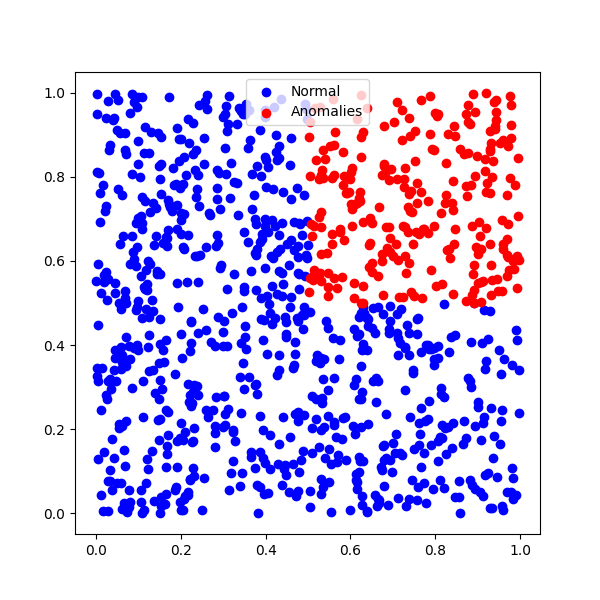
\includegraphics[width=0.3\textwidth]{images/norm_ano_ex.png}  % Replace with your image filename
    \caption{Example where two feature separate the normal and anomalous points better than either one alone.}
    \label{fig:two_feature_example}
\end{figure}

\bibliographystyle{plain}  % or IEEEtran, unsrt, etc.
\bibliography{references}
\end{document}
